\documentclass{standalone}
\usepackage{pgfplots}
\pgfplotsset{compat=1.16}
\begin{document}
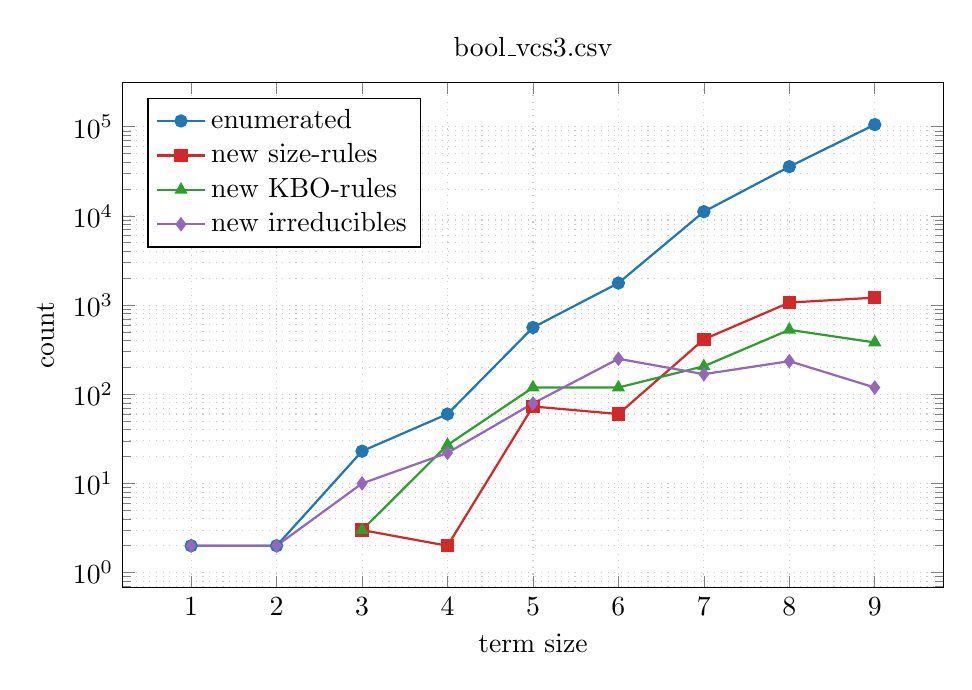
\begin{tikzpicture}
  \begin{axis}[
      width=12cm, height=8cm,
      xlabel={term size},
      ylabel={count},
      title={bool\_vcs3.csv},
      ymode=log,
      grid=both,
      grid style={dotted, gray!40},
      legend pos=north west,
      legend cell align=left,
      mark size=2pt,
    ]
    \definecolor{cenumerated}{HTML}{1f77b4}
    \addplot[color=cenumerated, mark=*, thick] coordinates {(1,2) (2,2) (3,23) (4,60) (5,561) (6,1767) (7,11154) (8,35689) (9,105706)};
    \addlegendentry{enumerated}
    \definecolor{cnewsizerules}{HTML}{d62728}
    \addplot[color=cnewsizerules, mark=square*, thick] coordinates {(1,0) (2,0) (3,3) (4,2) (5,73) (6,60) (7,413) (8,1067) (9,1212)};
    \addlegendentry{new size-rules}
    \definecolor{cnewkborules}{HTML}{2ca02c}
    \addplot[color=cnewkborules, mark=triangle*, thick] coordinates {(1,0) (2,0) (3,3) (4,27) (5,119) (6,119) (7,206) (8,528) (9,381)};
    \addlegendentry{new KBO-rules}
    \definecolor{cnewirreducibles}{HTML}{9467bd}
    \addplot[color=cnewirreducibles, mark=diamond*, thick] coordinates {(1,2) (2,2) (3,10) (4,22) (5,79) (6,250) (7,168) (8,235) (9,119)};
    \addlegendentry{new irreducibles}
  \end{axis}
\end{tikzpicture}
\end{document}
